\scanpage{360}
\hfill EZ 3

Les applications shuffles et A-W sont \uline{assoc}

et \uline{shuffles} est (anti)-commutative

(\quad A-W - est seulement comm à homotopie près

On peut exprimer ceci avec des diagrammes d'\unsure{objet|objets} trisimpliciaux

\margin{Ref \uline{Illusie}\quad\uline{thèse.}}
\diagram{\begin{tikzcd}[column sep=large]
X_{***}\arrow[r,"N_{\unsure{**|12}}"]\arrow[d,"\Delta_{12}"']&X_{\cdot\cdot\cdot}\arrow[r,"\int_{12}"]&X_{\cdot\cdot}\arrow[d,no head,"\int"]\\
X_{**}\arrow[r,"N"]&X_{\cdot\cdot}&X_{\cdot}
\end{tikzcd}}
\figure{\begin{tikzpicture}\draw (0,.15) .. controls (2,0) and (4,-.1) .. (6,-.5);\end{tikzpicture}}
Clair pour $\underbrace{ZX}$.

\deleted{$\unsure{ZX\otimes ZX|ZX\times ZX}\unsure{\longrightarrow}$}
\figure{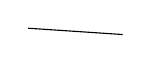
\begin{tikzpicture}\draw (0,0)--(1.2,-.08);\end{tikzpicture}}

L'énoncé de commutativité s'énonce comme suit.
\margin{$X$ ens simpl}

\deleted{$\operatorname{Hom}(ZX\otimes ZX,Z(X\times X))$}
\diagram{\begin{tikzcd}
\operatorname{Hom}^{\unsure{'|\bullet}}(Z(X\times X)^\sim,\widetilde{ZX}\otimes\widetilde{ZX})\arrow[r]&\mathbb Z
\end{tikzcd}}
\diagram{\begin{tikzcd}[column sep=large]
\text{\margin{$\Sigma_2$ agit sur ce complexe}}\arrow[r,bend right=12]&\operatorname{Hom}(Z(X_0\times X_0)\unsure{\not\to|\not\simeq}ZX_0\otimes ZX_0)\arrow[r]&Z
\end{tikzcd}}
\diagram{\begin{tikzcd}
X\arrow[r]&\mathrm{pt}\arrow[r,draw=none,"{\deleted{\longrightarrow}}" description]&{}
\end{tikzcd}}
\diagram{\begin{tikzcd}
\uline{\operatorname{Hom}(Z(,),\widetilde Z()\otimes\widetilde Z())}\arrow[r]&Z
\end{tikzcd}}

\uline{Théorème} (Dold): ``\unsure{Ueber|Über} Steenrodsche operationen --''

Pour tout $X$, ce complexe
\[
\left.\begin{gathered}
\operatorname{Hom}^{\unsure{'|\bullet}}(Z(X\ldots\times X),Z(X)\otimes\ldots\otimes ZX)\\
\operatorname{Hom}^{\unsure{'|\bullet}}(ZX\otimes\ldots\otimes ZX,Z(X\unsure{\times|,}\ldots\times X))
\end{gathered}\right\}
\]
est une résolution libre de $Z$ dans la cat des $\Sigma_n$-modules
\inserted{pour $X$ variable}

On tronque pour avoir un complexe de chaines
\mspage{361}
